%% For normal draft builds (figs undisplayed hence fast compile)
%\documentclass[hyperpdf,nobind,draft,oneside]{hepthesis}
%\documentclass[hyperpdf,nobind,draft,twoside]{hepthesis}

%% For short draft builds (breaks citations by necessity)
%\documentclass[hyperpdf,nobind,draft,hidefrontback]{hepthesis}

%%For Cambridge soft-bound version
\documentclass[hyperpdf,bindnopdf]{hepthesis}
%% For Cambridge hard-bound version (must be one-sided)
%\documentclass[hyperpdf,oneside]{hepthesis}

%% Load special font packages here if you wish
%\usepackage{lmodern}
\usepackage{mathpazo}
%\usepackage{euler}

%% Put package includes etc. into preamble.tex for convenience
\usepackage{xspace}
\usepackage{tikz}
%\usepackage{morefloats,subfig,afterpage}
\usepackage{mathrsfs} % script font
\usepackage{verbatim}
\usepackage{cite}
\usepackage{graphicx}
\usepackage{caption}
\usepackage{subcaption}

%% Load special font packages here if you wish
\usepackage{lmodern}  % lmodern, mathpazo, euler

%% Using Babel allows other languages to be used and mixed-in easily
\usepackage[english]{babel}
\selectlanguage{english}

%% Use the tikz-feynman package for Feynman diagram.
\usepackage[compat=1.1.0]{tikz-feynman}

%% Tweak so maths adapts its boldness to match the context.
\makeatletter
\g@addto@macro\bfseries\boldmath
\makeatother

%% Maths
\usepackage{resources/abmath}
\DeclareRobustCommand{\mymath}[1]{\ensuremath{\maybebmsf{#1}}}
% \DeclareRobustCommand{\parenths}[1]{\mymath{\left({#1}\right)}\xspace}
% \DeclareRobustCommand{\braces}[1]{\mymath{\left\{{#1}\right\}}\xspace}
% \DeclareRobustCommand{\angles}[1]{\mymath{\left\langle{#1}\right\rangle}\xspace}
% \DeclareRobustCommand{\sqbracs}[1]{\mymath{\left[{#1}\right]}\xspace}
% \DeclareRobustCommand{\mods}[1]{\mymath{\left\lvert{#1}\right\rvert}\xspace}
% \DeclareRobustCommand{\modsq}[1]{\mymath{\mods{#1}^2}\xspace}
% \DeclareRobustCommand{\dblmods}[1]{\mymath{\left\lVert{#1}\right\rVert}\xspace}
% \DeclareRobustCommand{\expOf}[1]{\mymath{\exp{\!\parenths{#1}}}\xspace}
% \DeclareRobustCommand{\eexp}[1]{\mymath{e^{#1}}\xspace}
% \DeclareRobustCommand{\plusquad}{\mymath{\oplus}\xspace}
% \DeclareRobustCommand{\logOf}[1]{\mymath{\log\!\parenths{#1}}\xspace}
% \DeclareRobustCommand{\lnOf}[1]{\mymath{\ln\!\parenths{#1}}\xspace}
% \DeclareRobustCommand{\ofOrder}[1]{\mymath{\mathcal{O}\parenths{#1}}\xspace}
% \DeclareRobustCommand{\SOgroup}[1]{\mymath{\mathup{SO}\parenths{#1}}\xspace}
% \DeclareRobustCommand{\SUgroup}[1]{\mymath{\mathup{SU}\parenths{#1}}\xspace}
% \DeclareRobustCommand{\Ugroup}[1]{\mymath{\mathup{U}\parenths{#1}}\xspace}
% \DeclareRobustCommand{\I}[1]{\mymath{\mathrm{i}}\xspace}
% \DeclareRobustCommand{\colvector}[1]{\mymath{\begin{pmatrix}#1\end{pmatrix}}\xspace}
\DeclareRobustCommand{\Rate}{\mymath{\Gamma}\xspace}
\DeclareRobustCommand{\RateOf}[1]{\mymath{\Gamma}\parenths{#1}\xspace}

%% High-energy physics stuff
\usepackage{resources/abhep}
%\usepackage{resources/SIunits}
%\usepackage{hepnames}
%\usepackage{hepunits}

\begin{comment}
TODO: cross-section, nu and nu bar combos, proton, neutron, electron, muon, tau etc
\end{comment}

% Use \xspace at the end of the macros
% Use \text for text of units in macro
% write 5--10 for 5 to 10
% \mathrm{...} macro, i.e. $\mathrm{d}f/\mathrm{d}x$ → df /dx, not $df/dx$ → df /dx
% So put the whole of each mathematical expression in math mode (and drop out of it via \mathrm or \text if needed).
% Negative numbers should be written in math mode
% always wrap text in your equations in the \mathrm macro, which does it right

%% Personal macros
\DeclareRobustCommand{\chips}{\textsc{Chips}\xspace}
\DeclareRobustCommand{\chipsm}{\textsc{Chips-M}\xspace}
\DeclareRobustCommand{\chipsfive}{\textsc{Chips-5}\xspace}
\DeclareRobustCommand{\nova}{NOvA\xspace}
\DeclareRobustCommand{\minos}{\textsc{Minos}\xspace}
\DeclareRobustCommand{\numi}{NuMI\xspace}
% GENIE
% ROOT
% Tensorflow
% Python
% Google
% 
%\newcommand{\eV}{\text{e\kern-0.15ex V}\xspace}
%\newcommand{\MeV}{\text{M\eV}\xspace}
%\newcommand{\GeV}{\text{G\eV}\xspace}
%\newcommand{\TeV}{\text{T\kern-0.1ex \eV}\xspace}


\DeclareRobustCommand{\arXivCode}[1]{arXiv:#1}
\DeclareRobustCommand{\CP}{\ensuremath{\mathcal{CP}}\xspace}
\DeclareRobustCommand{\CPviolation}{\CP-violation\xspace}
\DeclareRobustCommand{\CPv}{\CPviolation}
\DeclareRobustCommand{\LHC}{LHC\xspace}
\DeclareRobustCommand{\CERN}{CERN\xspace}
\DeclareRobustCommand{\bphysics}{\Pbottom-physics\xspace}
\DeclareRobustCommand{\bhadron}{\Pbottom-hadron\xspace}
\DeclareRobustCommand{\Bmeson}{\PB-meson\xspace}
\DeclareRobustCommand{\bbaryon}{\Pbottom-baryon\xspace}
\DeclareRobustCommand{\Bdecay}{\PB-decay\xspace}
\DeclareRobustCommand{\bdecay}{\Pbottom-decay\xspace}
\DeclareRobustCommand{\BToKPi}{\HepProcess{ \PB \to \PK \Ppi }\xspace}
\DeclareRobustCommand{\BToPiPi}{\HepProcess{ \PB \to \Ppi \Ppi }\xspace}
\DeclareRobustCommand{\BToKK}{\HepProcess{ \PB \to \PK \PK }\xspace}
\DeclareRobustCommand{\BToRhoPi}{\HepProcess{ \PB \to \Prho \Ppi }\xspace}
\DeclareRobustCommand{\BToRhoRho}{\HepProcess{ \PB \to \Prho \Prho }\xspace}
\DeclareRobustCommand{\X}{\thesismath{X}\xspace}
\DeclareRobustCommand{\Xbar}{\thesismath{\overline{X}}\xspace}
\DeclareRobustCommand{\Xzero}{\HepGenParticle{X}{}{0}\xspace}
\DeclareRobustCommand{\Xzerobar}{\HepGenAntiParticle{X}{}{0}\xspace}
\DeclareRobustCommand{\epluseminus}{\Ppositron\!\Pelectron\xspace}
\DeclareRobustCommand{\protonproton}{\Pproton\APantiproton\xspace}


%% You can set the line spacing this way
%\setallspacing{double}
%% or a section at a time like this
%\setfrontmatterspacing{double}


%% Define the thesis title and author
\title{Deep Convolution Neural Networks for the CHIPS Experiment}
\author{Josh Chalcraft Tingey}

%% Doc-specific PDF metadata
\makeatletter
\@ifpackageloaded{hyperref}{%
\hypersetup{%
  pdftitle = {Deep Convolution Neural Networks for the CHIPS Experiment},
  pdfsubject = {Josh Tingey's PhD thesis},
  pdfkeywords = {CHIPS, physics, CNN, Machine Learning},
  pdfauthor = {\textcopyright\ Josh Tingey}
}}{}
\makeatother

%% Start the document
\begin{document}

%% Define the un-numbered front matter (cover pages, rubrik and table of contents)
\begin{frontmatter}
  %% Title
\titlepage[of University College London]{%
  A dissertation submitted to University College London\\ for the degree of Doctor of Philosophy}

%% Abstract
\begin{abstract}%[\smaller \thetitle\\ \vspace*{1cm} \smaller {\theauthor}]
  %\thispagestyle{empty}
  \LHCb is a \bphysics detector experiment which will take data at
  the \unit{14}{\TeV} \LHC accelerator at \CERN from 2007 onward\dots
\end{abstract}


%% Declaration
\begin{declaration}
  This dissertation is the result of my own work, except where explicit
  reference is made to the work of others, and has not been submitted
  for another qualification to this or any other university. This
  dissertation does not exceed the word limit for the respective Degree
  Committee.
  \vspace*{1cm}
  \begin{flushright}
    Andy Buckley
  \end{flushright}
\end{declaration}


%% Acknowledgements
\begin{acknowledgements}
  Of the many people who deserve thanks, some are particularly prominent,
  such as my supervisor\dots
\end{acknowledgements}


%% Preface
\begin{preface}
  This thesis describes my research on various aspects of the \LHCb
  particle physics program, centred around the \LHCb detector and \LHC
  accelerator at \CERN in Geneva.

  \noindent
  For this example, I'll just mention \ChapterRef{chap:SomeStuff}
  and \ChapterRef{chap:MoreStuff}.
\end{preface}

%% ToC
\tableofcontents


%% Strictly optional!
\frontquote{%
  Writing in English is the most ingenious torture\\
  ever devised for sins committed in previous lives.}%
  {James Joyce}
%% I don't want a page number on the following blank page either.
\thispagestyle{empty}

\end{frontmatter}

%% Start the content body of the thesis
\begin{mainmatter}
  %% Actually, more semantic chapter filenames are better, like "chap-bgtheory.tex"
  \chapter{Introduction}
\label{chap:introduction}

%% Restart the numbering to make sure that this is definitely page #1!
\pagenumbering{arabic}

blah blah blah
  \chapter{Theory}
\label{chap:theory}

%% Note that the citations in this chapter use the journal and
%% arXiv keys: I used the SLAC-SPIRES online BibTeX retriever
%% to build my bibliography. There are also quite a few non-standard
%% macros, which come from my personal collection. You can have them
%% if you want, or I might get round to properly releasing them at
%% some point myself.

\chapterquote{Laws were made to be broken.}%
{Christopher North, 1785--1854}%: Blackwood's Magazine May 1830

Symmetries, either intact or broken, have proved to be at the heart
of how matter interacts. The Standard Model of fundamental interactions
(SM) is composed of three independent continuous symmetry groups denoted
$\SUgroup{3} \times \SUgroup{2} \times \Ugroup{1}$, representing the
strong force, weak isospin and hypercharge
respectively~\cite{Phys.Rev.Lett.19.1264, Phys.Rev.D2.1285,hep-ph/0410370}.

\section{Neutral meson mixing}
\label{sec:neutralmixing}
We can go a long way with an effective Hamiltonian approach in
canonical single-particle quantum mechanics. To do this we construct
a wavefunction from a combination of a generic neutral meson state
$\ket{\Xzero}$ and its anti-state $\ket{\Xzerobar}$:
%
\begin{equation}
  \ket{\psi(t)} = a(t)\ket{\Xzero} + b(t)\ket{\Xzerobar}
\end{equation}
%
which is governed by a time-dependent matrix differential equation,
%
\begin{equation}
  \I \pdByd{}{t} \colvector{a \\ b}
  =
  \underbrace{%
  \twomatrix{ M_{11}-\frac{\I}{2}\Gamma_{11}
            & M_{12}-\frac{\I}{2}\Gamma_{12} }
            { M_{12}^\ast-\frac{\I}{2}\Gamma_{12}^\ast
            & M_{22}-\frac{\I}{2}\Gamma_{22} }
  }_{\boldmatrix{H}}
  \colvector{a \\ b}
  .
\end{equation}

  \chapter{The CHIPS experiment}
\label{chap:chips}

\chapterquote{There, sir! that is the perfection of vessels!}
{Jules Verne, 1828--1905}

\section{The \LHC}
The Large Hadron Collider (\LHC) at \CERN is a new hadron collider,
located in the same tunnel as the Large Electron-Positron collider
(\LEP)~\cite{Brianti:2004qq}. Where \LEP's chief task was the use
of \unit{90--207}{\GeV} \epluseminus collisions to establish the
precision physics of electroweak unification\dots

\begin{figure}
  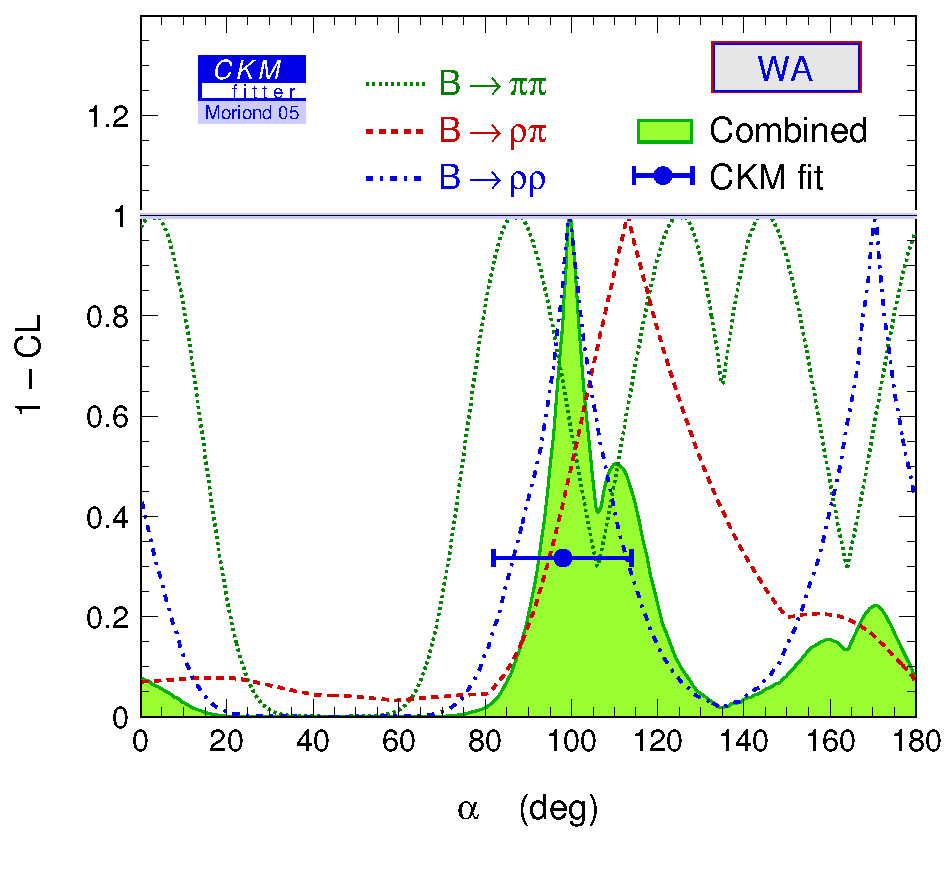
\includegraphics[width=\largefigwidth]{diagrams/3_chips/ckmfitter-alpha-combined}
  \caption[CKM Fitter constraints on \alphaCKM.]%
  {CKM Fitter constraints on \alphaCKM from combined \BToPiPi,
    \BToRhoPi and \BToRhoRho decay analyses.}
  \label{fig:CKMFitter}
\end{figure}

\section{The \LHCb experiment}
\label{sec:LHCbInDetail}

Since both \bhadron{s} are preferentially produced in the same direction
and are forward-boosted along the beam-pipe, the detector is not required
to have full $4\pi$ solid-angle coverage. \LHCb takes advantage of this
by using a wedge-shaped single-arm detector with angular acceptance
\unit{10-300}{\mrad} in the horizontal (bending) plane~\cite{Amato:1998xt}.

\vspace{1cm}

\begin{center}
{\hspace{1mm}\Large\vdots\hspace{1cm}}
\end{center}

\vspace{1cm}

The detector is illustrated in \FigureRef{fig:LHCbCrossSection}, showing
the overall scale of the experiment and the surrounding cavern structure.

\begin{sidewaysfigure}
  \begin{center}
  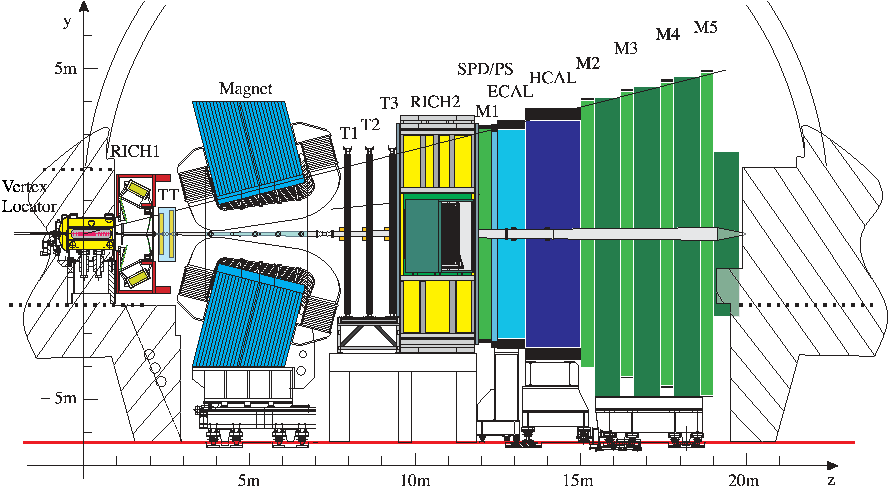
\includegraphics[width=0.8\textheight]{diagrams/3_chips/lhcb-detector-cross-section}
  \caption[Cross-section view of \LHCb, cut in the non-bending $y$--$z$ plane]%
    {Cross-section view of \LHCb, cut in the non-bending $y$--$z$ plane.}
  \label{fig:LHCbCrossSection}
  \end{center}
\end{sidewaysfigure}

The single-sided detector design was chosen in preference to a two-armed
design since the detector dimensions are restricted by the layout of the
IP8 (ex-Delphi) cavern in which \LHCb is located. Using all the available
space for a single-arm spectrometer more than compensates in performance
for the \about{50\percent} drop in luminosity.

\section{The \Cerenkov mechanism}
A Huygens construction in terms of spherical shells of probability for photon
emission as the particle progresses along its track shows an effective
``shock-front'' of \Cerenkov emission. This corresponds to an emission cone of
opening angle \thetaCerenkov around the momentum vector for each point on the
track,
%
\begin{subequations}
  \label{eq:cosThetaCk}
  \begin{equation}
    \cos\,\thetaCerenkov  &= \frac{1}{n \beta} +
                             \frac{\hbar k}{2p}%
                             \parenths{ 1 - \frac{1}{n^2} } \\
                          &\,\sim \frac{1}{n \beta}%
    \label{eq:cosThetaCkApprox}
  \end{equation}
\end{subequations}
%
where $\beta \equiv v/c$, the relativistic velocity fraction.

\section{Trigger system}
\label{sec:triggers}
An overview of the \LHCb trigger characteristics broken down by level
is shown in \Table~\ref{tab:TriggerDetails}.

\begin{table}[bp]
  \begin{tabular}{lllll}
                & L0              & L1              & HLT             \\
    \midrule\\
    Input rate  & \unit{40}{\MHz} & \unit{1}{\MHz}  & \unit{40}{\kHz} \\
    Output rate & \unit{1}{\MHz}  & \unit{40}{\kHz} & \unit{2}{\kHz}  \\
    Location    & On detector     & Counting room   & Counting room   \\
  \end{tabular}
  \caption{Characteristics of the trigger levels and offline analysis.}
  \label{tab:TriggerDetails}
\end{table}

  \chapter{DAQ}
\label{chap:daq}

Here are some funky floats using ``continued captions'', i.e. for a semantically
collected group of float contents which are too numerous to fit into a single
float, such as the pretty circles in the following figure:

\newcommand{\circleimg}[1]{%
\begin{tikzpicture}
  \draw[color=black,fill=#1,thick] (1,0) circle (1.5cm);
\end{tikzpicture}%
}

\begin{figure}[hb]
  \subfloat[][Example 1a]{\label{fig:cc1a}\circleimg{red!80}}\quad
  \subfloat[][Example 1b]{\label{fig:cc1b}\circleimg{green!70!yellow}}\quad
  \subfloat[][Example 1c]{\label{fig:cc1c}\circleimg{blue!80}}\quad
  \subfloat[][Example 1d]{\label{fig:cc1d}\circleimg{orange!80!yellow}}
  \caption{Demonstration of \texttt{subfig} continued captions.}
  \label{fig:cc1}
\end{figure}

\begin{figure}[p]
  \ContinuedFloat
  \subfloat[][Example 1e]{\label{fig:cc1e}\circleimg{violet}}\quad
  \subfloat[][Example 1f]{\label{fig:cc1f}\circleimg{cyan}}\quad
  \subfloat[][Example 1g]{\label{fig:cc1g}\circleimg{magenta}}\quad
  \subfloat[][Example 1h]{\label{fig:cc1h}\circleimg{yellow}}
  \caption[]{Demonstration of \texttt{subfig} continued captions (continued).}
\end{figure}

\noindent
This mechanism means that the same float label is used for both pages of
floats. Note that we can refer to \FigureRef{fig:cc1} in general, or to
\FigureRef{fig:cc1g} on \PageRef{fig:cc1g} in particular!

\noindent
Just for the hell of it, let's also refer to \SectionRef{sec:neutralmixing}.

  \chapter{CVN}
\label{chap:cvn}

Here are some funky floats using ``continued captions'', i.e. for a semantically
collected group of float contents which are too numerous to fit into a single
float, such as the pretty circles in the following figure
  \chapter{Results}
\label{chap:results}

Here are some funky floats using ``continued captions'', i.e. for a semantically
collected group of float contents which are too numerous to fit into a single
float, such as the pretty circles in the following figure
  \chapter{Cosmics}
\label{chap:cosmics}

Here are some funky floats using ``continued captions'', i.e. for a semantically
collected group of float contents which are too numerous to fit into a single
float, such as the pretty circles in the following figure blah blah blah
  \chapter{Conclusion}
\label{chap:conclusion}

Here are some funky floats using ``continued captions'', i.e. for a semantically
collected group of float contents which are too numerous to fit into a single
float, such as the pretty circles in the following figure
  %% To ignore a specific chapter while working on another, making the build faster, comment it out:
  %\input{chap4}
\end{mainmatter}

%% Produce the appendices
\begin{appendices}
  %% The "\appendix" call has already been made in the declaration
%% of the "appendices" environment (see thesis.tex).
\chapter{Pointless extras}
\label{app:Pointless}

\chapterquote{%
Le savant n'\'etudie pas la nature parce que cela est utile; \\
\indent il l'\'etudie parce qu'il y prend plaisir, \\
\indent et il y prend plaisir parce qu'elle est belle.}%
{Henri Poincar\'e, 1854--1912}

Appendixes (or should that be ``appendices''?) make you look really clever, 'cos
it's like you had more clever stuff to say than could be fitted into the main
bit of your thesis. Yeah. So everyone should have at least three of them\dots

\section{Like, duh}
\label{sec:Duh}
Padding? What do you mean?

\section{$y = \alpha x^2$}
\label{sec:EqnTitle}
See, maths in titles automatically goes bold where it should (and check the
table of contents: it \emph{isn't} bold there!) Check the source: nothing
needs to be specified to make this work. Thanks to Donald Arsenau for the
teeny hack that makes this work.

%% Big appendixes should be split off into separate files, just like chapters
%\input{app-myreallybigappendix}

\end{appendices}

%% Produce the un-numbered back matter (e.g. colophon,
%% bibliography, tables of figures etc., index...)
\begin{backmatter}
  \begin{colophon}
  This thesis was made in \LaTeXe{} using the ``hepthesis'' class~\cite{hepthesis}.
\end{colophon}

%% You're recommended to use the eprint-aware biblio styles which
%% can be obtained from e.g. www.arxiv.org. The file mythesis.bib
%% is derived from the source using the SPIRES Bibtex service.
\bibliographystyle{h-physrev}
\bibliography{mythesis}

%% I prefer to put these tables here rather than making the
%% front matter seemingly interminable. No-one cares, anyway!
\listoffigures
\listoftables

%% If you have time and interest to generate a (decent) index,
%% then you've clearly spent more time on the write-up than the 
%% research ;-)
%\printindex

\end{backmatter}

%% Close
\end{document}
